\subsection{The Challenges of Monitoring}
Consider the following examples of commonplace automated tasks in three different application domains:
\begin{enumerate}
\item An automated stock market trading system monitors the distribution of buy and sell orders of a particular stock to identify the best time and price for its own orders.
\item A corporate data warehouse monitors the current status of its production facilities, warehoused inventory and active demand for its products in order to preemptively identify supply chain problems.
\item A compute cluster monitors its current status overnight to alert a network administrator when some of its hardware fails, but only if the chance of computations being disrupted by further failures exceeds a given threshold.
\end{enumerate}

The core challenge in automating each of these tasks is the instantiation of a system for {\em monitoring} the state of the world from the application domain's perspective, be it a stock market, data warehouse, or compute cluster, etc\ldots.  This is a fundamentally data-management challenge: As the state of the world changes, the monitoring system must update it's own internal view of that state accordingly -- each order placed for a given stock can potentially affect the automated trading system's behavior.  

In spite of this, the challenges associated with monitoring rapidly changing, but otherwise persistent state have not been sufficiently addressed by the database community. Although active database (i.e., Triggers)\cite{?} and complex stream event processing (CEP)\cite{?} techniques both address the challenges of monitoring persistent state, neither is designed to handle complexity in the monitoring task, nor rapid changes to ``persistent'' state.  In this section we now support this assertion through experimental (and some anecdotal) evidence, which clearly demonstrates that existing data-management systems are incapable of efficiently performing these sorts of monitoring tasks.

We consider the three example scenarios as described above.  Each monitoring task is implemented using triggers in Postgres and two commercial database systems, and using CEP in two commercial stream processing systems\footnote{The names of the commercial databases and stream processors are kept anonymous due to restrictions in their license agreements.}.  Concretely, the scenarios are as follows:

\begin{figure}
\tinysection{Example \ref{ex:dbfail:stock}}
\begin{verbatim}
-- Example 2.1 --
CREATE TABLE bids(volume float, price float);
CREATE TABLE asks(volume float, price float);
\end{verbatim}

\tinysection{Example \ref{ex:dbfail:tpch}}'s schema is identical to the TPC-H schema\cite{tpch}.

\tinysection{Example \ref{ex:dbfail:network}}
\begin{verbatim}
CREATE TABLE Server(ssid int, status int);
CREATE TABLE Task(ttid int, priority int);
CREATE TABLE Assignment(asid int, atid int);
\end{verbatim}

\label{fig:dbfail:schemas}
\caption{Schemas for the three example scenarios}
\end{figure}

\begin{example}
\label{ex:dbfail:stock}
A stock market trading system monitors the spread across significant orders for a particular stock (i.e., orders larger than 0.01\% of the total volume of orders for the stock).  Given the table schemas defined in Figure \ref{fig:dbfail:example:schemas}, we can express the value being monitored as a SQL query:
% test/sql/finance/pricespread.sql
\begin{verbatim}
SELECT SUM(a.price - b.price)
FROM   bids b, asks a
WHERE  b.volume > 0.0001 * (SELECT SUM(b1.volume) 
                            FROM   bids b1)
  AND  a.volume > 0.0001 * (SELECT SUM(a1.volume) 
                            FROM   asks a1);
\end{verbatim}
\end{example}

\begin{example}
\label{ex:dbfail:tpch}
A corporate data warehouse monitors the volume of of parts of each type being shipped between each region based on the locations of the supplier and the client.  Given the standard TPC-H benchmark schema\cite{tpch}, we can express this monitoring task as the following SQL group-by query (based on, but not identical to SSB query 4\cite{ssb}): 
\begin{verbatim}
SELECT   sn.regionkey, cn.regionkey,
         p.type, SUM(li.quantity)
FROM     CUSTOMER c, ORDERS o, LINEITEM li, PART p, 
         SUPPLIER s, NATION cn, NATION sn
WHERE       c.custkey = o.custkey
  AND      o.orderkey = li.orderkey
  AND       p.partkey = li.partkey
  AND       s.suppkey = li.suppkey
  AND    cn.nationkey = c.nationkey
  AND    sn.nationkey = s.nationkey
GROUP BY sn.regionkey, cn.regionkey, PART.type;
\end{verbatim}
\end{example}

\begin{example}
\label{ex:dbfail:network}
A cluster monitoring system keeps monitors servers assigned to work on different compute tasks -- the system issues an alert whenever the number of failed servers assigned to a given task exceeds a given threshold (e.g., 50\%).  These alerts are dispatched based on priority, and number of threatened tasks.  Given the table schemas defined in Figure \ref{fig:dbfail:example:schemas}, we can represent this monitoring task as triggering whenever the following SQL group-by query returns a non-empty result:
\begin{verbatim}
SELECT priority, COUNT(*)
FROM   Task t
WHERE  (SELECT COUNT(*) 
        FROM Assignment a2,Server s2
        WHERE t.ttid = a2.atid 
        AND a2.asid = s2.ssid) * 0.5 > 
       (SELECT COUNT(*) 
        FROM Assignment a3,Server s3
        WHERE t.ttid = a3.atid 
        AND a3.asid = s3.ssid 
        AND s3.status = 1)
GROUP BY t.priority;
\end{verbatim}
\end{example}

\subsection{Monitoring with Active Databases}
The first existing technique for monitoring in the database literature is based around so called Active Databases\cite{?}.  This technique allows user-defined {\em triggers} to intercept updates to one table in the database, and initiate secondary updates as a result.  Trigger functionality has been implemented in most high-end database management systems -- Postgres\cite{?}, MySQL\cite{?}, and virtually all commercial systems, including the two we test.

Closely related to Active Databases are Incremental View Maintenance\cite{?} (IVM) systems.  Rather than allowing arbitrary user-defined operations to trigger after updates to the database, IVM systems allow users to define materialized views.  The result of the view query is materialized, but rather than re-evaluating the entire query from scratch whenever one of the tables in the query changes, the IVM system uses a so-called delta query.  The delta query is a simpler form of the original query, which identify how the original query changes as after an update to one of its tables.  

\begin{example}
For example, consider the query from Example \ref{ex:dbfail:tpch} and an insertion into the {\tt LINEITEM} table:
\begin{verbatim}
INSERT INTO 
LINEITEM(orderkey, partkey, suppkey, quantity)
VALUES  (37,       42,      7,       100);
\end{verbatim}

We can run the following query:
\begin{verbatim}
SELECT   sn.regionkey, cn.regionkey,
         p.type, SUM(100)
FROM     CUSTOMER c, ORDERS o, PART p, 
         SUPPLIER s, NATION cn, NATION sn
WHERE       c.custkey = o.custkey
  AND      o.orderkey = 37
  AND       p.partkey = 42
  AND       s.suppkey = 7
  AND    cn.nationkey = c.nationkey
  AND    sn.nationkey = s.nationkey
GROUP BY sn.regionkey, cn.regionkey, PART.type;
\end{verbatim}

Note that all columns from {\tt LINEITEM} have been replaced by the corresponding value being inserted.  The result of running this query is the delta to the original table.  The delta is then merged into the original query's materialized results -- group by terms are paired with like values from the original query, and the new sums are added to the corresponding old ones.  After merging in the delta, the materialized view correctly represents the results of the original query after the insertion into {\tt LINEITEM}.
\end{example}

Because the delta query is simpler, it can be evaluated more efficiently than the original, conceivably saving time on updates.  IVM functionality has been implemented into most commercial database systems, including the two we test.

\begin{figure*}
\begin{center}
\begin{tabular}{ccc}
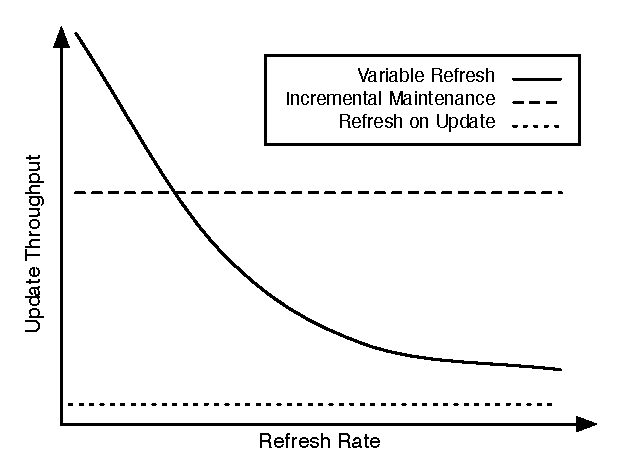
\includegraphics[width=2in]{../graphics-tmp/placeholder_db_result} &
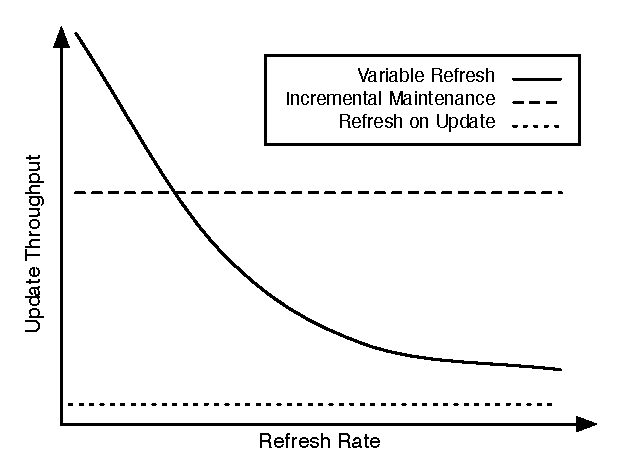
\includegraphics[width=2in]{../graphics-tmp/placeholder_db_result} &
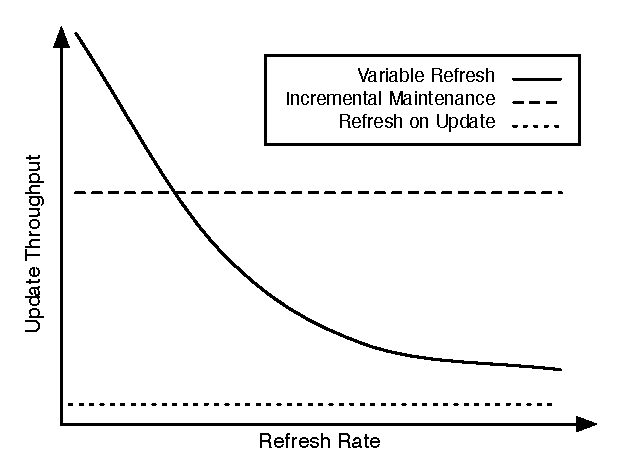
\includegraphics[width=2in]{../graphics-tmp/placeholder_db_result} \\
(a) & (b) & (c)
\end{tabular}
\end{center}
\label{fig:dbfail:postgres}
\caption{Performance results for Postgres on Examples \ref{ex:dbfail:stock} (a), \ref{ex:dbfail:tpch} (b), and \ref{ex:dbfail:network} (c).}
\end{figure*}
\begin{figure*}
\begin{center}
\begin{tabular}{ccc}
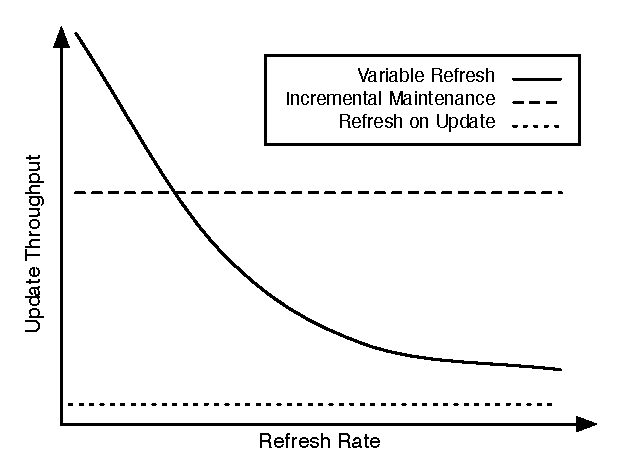
\includegraphics[width=2in]{../graphics-tmp/placeholder_db_result} &
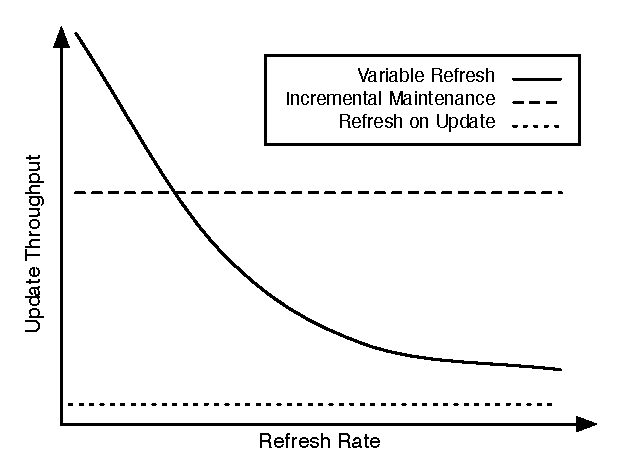
\includegraphics[width=2in]{../graphics-tmp/placeholder_db_result} &
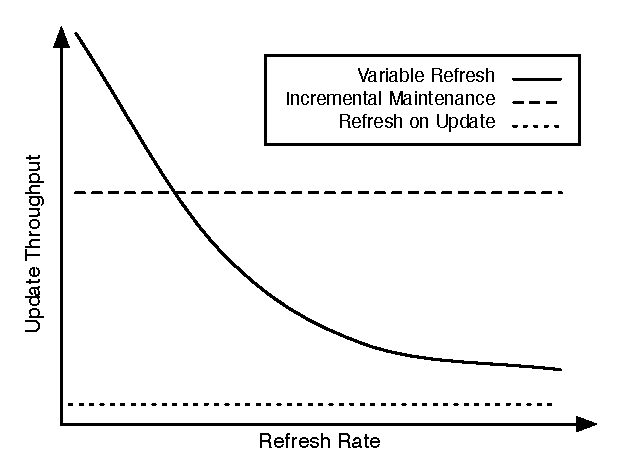
\includegraphics[width=2in]{../graphics-tmp/placeholder_db_result} \\
(a) & (b) & (c)
\end{tabular}
\end{center}
\label{fig:dbfail:CD1}
\caption{Performance results for Commercial DBMS 1 on Examples \ref{ex:dbfail:stock} (a), \ref{ex:dbfail:tpch} (b), and \ref{ex:dbfail:network} (c).}
\end{figure*}\begin{figure*}
\begin{center}
\begin{tabular}{ccc}
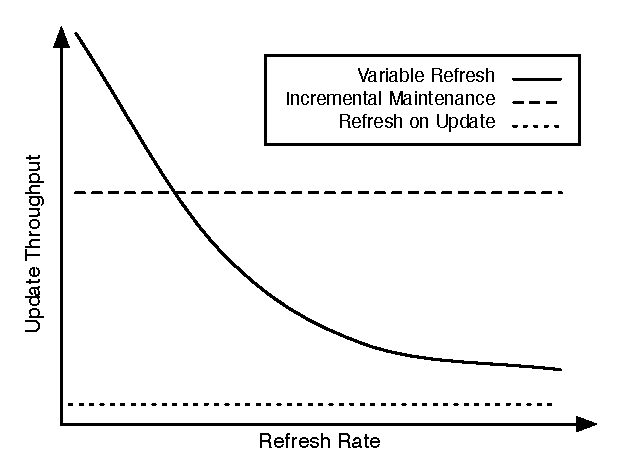
\includegraphics[width=2in]{../graphics-tmp/placeholder_db_result} &
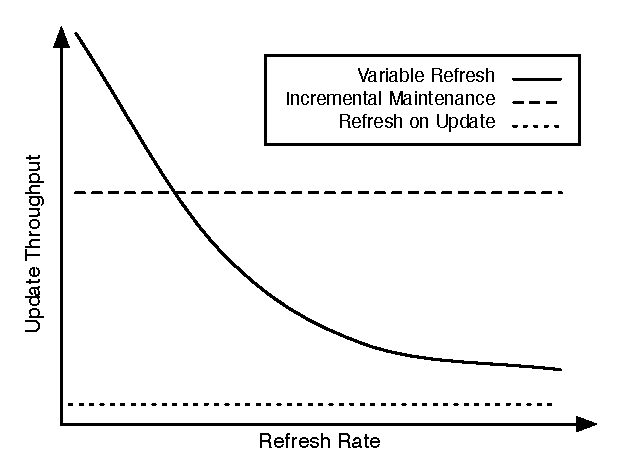
\includegraphics[width=2in]{../graphics-tmp/placeholder_db_result} &
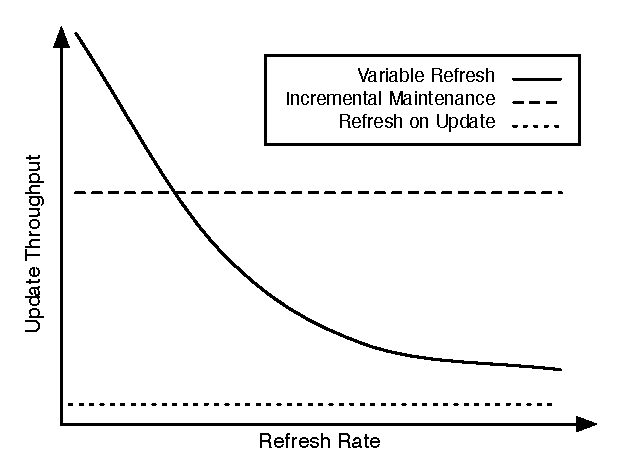
\includegraphics[width=2in]{../graphics-tmp/placeholder_db_result} \\
(a) & (b) & (c)
\end{tabular}
\end{center}
\label{fig:dbfail:CD2}
\caption{Performance results for Commercial DBMS 2 on Examples \ref{ex:dbfail:stock} (a), \ref{ex:dbfail:tpch} (b), and \ref{ex:dbfail:network} (c).}
\end{figure*}



\subsection{Monitoring with Stream Processors}

\subsection{Analysis}